\chapter{Adverting and Pricing Integration}

\setcounter{equ}{2}

Reached this point the goal is to attract the most valuable users, that is allocate the budget during Advertising so that it is focused on attracting users that will maximize the total reward; this expectation on the reward is modeled by the pricing algorithms presented before. In this section we will present how we have modeled the integration between Pricing and Advertising section, which are the algorithm proposed and an analysis of the final results.


\section{Proposed Integration}
The idea behind our integration is to have, for each Subcampaign, the possibility to manage separately the Advertising and the Pricing in order to reuse all the algorithms presented in the previous sections and, on top of it, build a Budget Allocator that is able to collect all the information and calculate the best allocation of the budget by solving the Knapsack Optimization Problem (Equation \ref{equ:knapsack}).
The complete flow chart can be found at Figure \ref{fig:part6scheme}, in the following sections we will discuss it step by step.

\subsection{Budget Allocator}
Every day, this component is the one that, collected information from the past, calculates the best budget allocation. Initially, when we have no historical information, it is built to output a balanced allocation among all the Subcampaigns. After the initialization phase, every new day, it collects for every subcampaign $ j $ two values:

\begin{enumerate}
    \item $ n_j (.) $ : Learned distribution of clicks over budget allocation for subcampaign$_j$. This function comes from the regression generated by the GPTS learner in the   \textbf{Advertising} section.
    \item $ v_j $ : Learned value, in terms of expected reward for subcampaign$_j$. This value comes from the evaluation of the collected reward during the last days in the \textbf{Pricing} section.
\end{enumerate}

At this point we are able to define the Knapsack Optimization Problem as:

\begin{equ}[!ht]
    \begin{equation*}
        \max_{y_j,_t} \sum_{j=1}^{N} v_j n_j(y_j,_t)
    \end{equation*}
    \begin{equation*}
        \sum_{j=1}^{N} y_j,_t \leq \bar{y}_t
    \end{equation*}
    \caption{The complete legend can be found at Figure \ref{fig:part6scheme}}
    \label{equ:knapsack}
\end{equ}

\subsection{Advertising}
For each subcampaign$_j$, given the budget allocation $ y_j,_t $, it is possible to collect from the environment the real number of clicks $ N_j(y_j,_t) $ generated by this allocation and update ,as we done in chapter 2 and 3, the \textit{Gaussian Process (GP) Learner}.
At the end it is returned the distribution $ n_j(.) $ learned by the GP.



\begin{figure}[H]
    \centering
    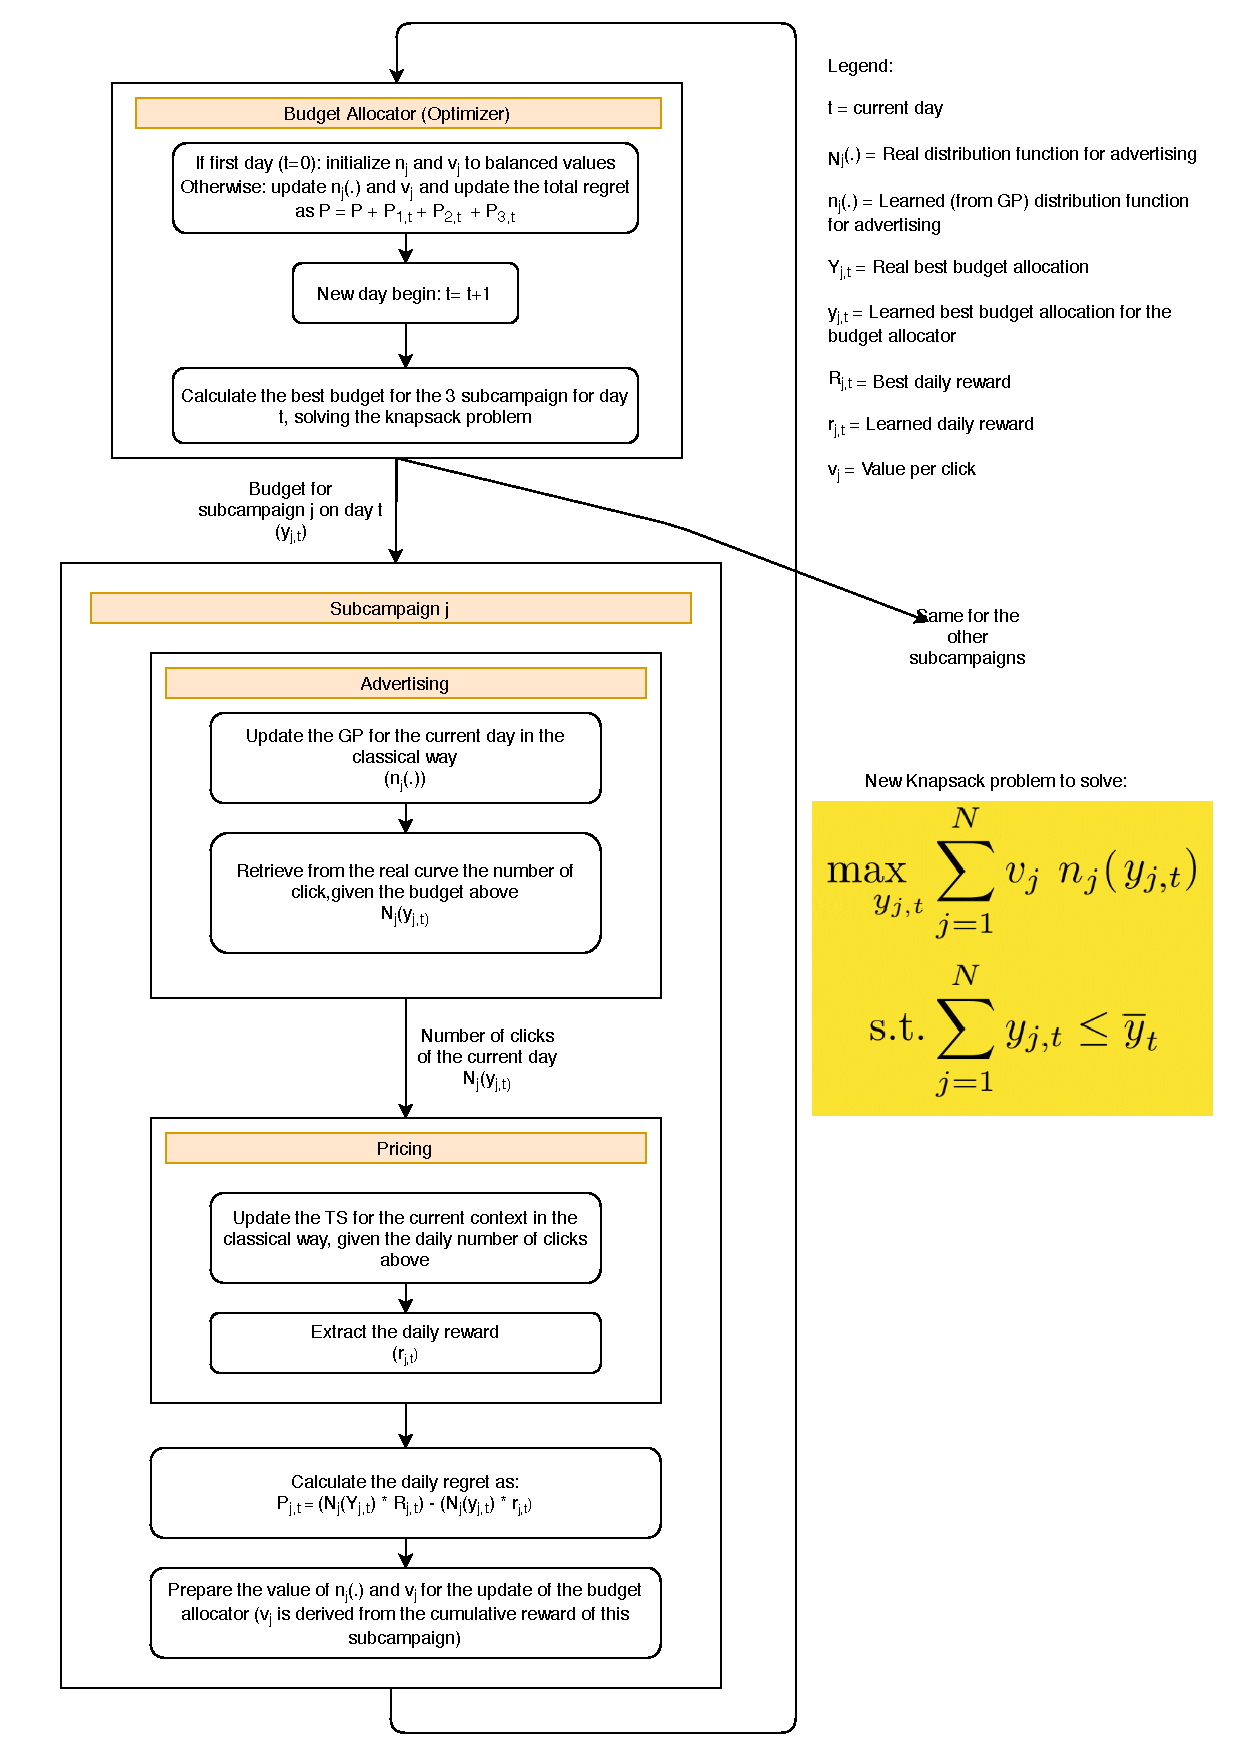
\includegraphics[scale=0.8]{images/part6_schema.pdf}
    \caption{Flow Chart Diagram of part 6}
    \label{fig:part6scheme}
\end{figure}

\subsection{Pricing}
For each subcampaign$_j$, given the real number of clicks $ N_j(y_j,_t) $ generated by the \textbf{Advertising}, it is possible to collect the real revenue $ r_j,_t $ for the current day and update, as we have done in Chapter 4, the \textit{Thompson Sampling (TS) Learner}. At the end it also returns the value $ v_j $ of this subcapmpaign, by averaging the collected revenue of the last N days. The reason of this choice is that we want to balance the trade-off between exploration (few days) and exploitation (more days). After validation runs we have chosen N=5 days.


\section{Performance Evaluation}
At the end of each day, given $ r_j,_t $ and $ R_j,_t $, the optimal daily reward, the regret of the current day for every subcampaign is calculated. As in Chapter 4 and 5, we configured the experiment to both keep the same price for the day and not to and this is the reason of the two graphs. It is possible to see that, in agreement of what presented before, the regret in which is proposed different prices for each visit is smaller than the opposite case. \ref{fig:regret6Fig}.\\
We have also evaluated the final loss, calculated as the total regret divided by the cumulative clairvoyant reward, that is around 2.64\%, while the loss of the version with keeping price fixed is 4.47\%. \\

\begin{figure}[!htb]
    \centering

    \begin{subfigure}[!H]{0.8\textwidth}
        \centering
        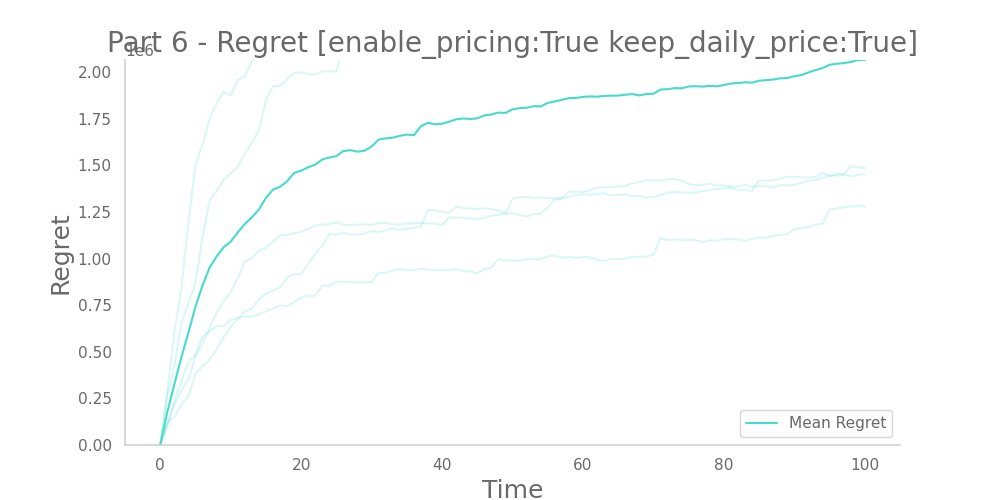
\includegraphics[width=\textwidth]{images/part6_enable-pricingTrue_keep-daily-priceTrue.png}
        \caption{Regret obtained proposing to the customers the same price for the entire day.}
    \end{subfigure}

    \begin{subfigure}[!H]{0.8\textwidth}
        \centering
        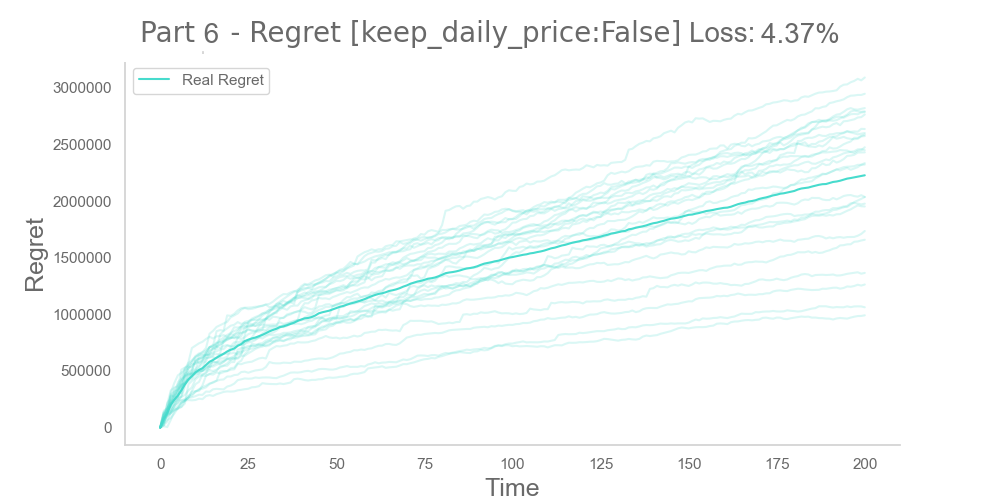
\includegraphics[width=\textwidth]{images/part6_enable-pricingTrue_keep-daily-priceFalse.png}
        \caption{Regret obtained proposing to the customers different prices for each visit.}
    \end{subfigure}
    \caption{Comparison between the regrets obtained during the campaign.}
    \label{fig:regret6Fig}
\end{figure}




